\section{results}

The objective function of the genetic algorithm is the accuracy of the model. Therefore, for each generation member, the model must be trained, and the accuracy of the model must be determined, which makes the computational cost very high. A method has been used to reduce the computational cost as much as possible. A filter is placed in the objective function whose job is to detect duplicate inputs. If the input is duplicated and the model has already been trained with the same structure, the algorithm searches for the corresponding answer among the previous answers and records it as the objective function's output.
The research algorithm is written in Python programming language on the Tensorflow framework and the Keras library. The test runs on a computer with a 3.2GHz CPU, 32GB RAM \&  NVIDIA GeForce GTX 1080 specifications.

% ------------------------------------------------------ %
%% Please add the following required packages to your document preamble:
% \usepackage{multirow}
% \usepackage{longtable}
% Note: It may be necessary to compile the document several times to get a multi-page table to line up properly

\begin{longtable}{cccccccccc}
\caption{confusion matrix of the original model}
\label{tab:my-table}\\
\cline{2-10}
                        & \multicolumn{9}{c}{Predicted}                      \\ \cline{2-10} 
\endfirsthead
%
\endhead
%
                        &    & G0  & G1  & G2  & G3  & G4  & G5  & G6  & G7  \\ \hline
\multirow{8}{*}{Actual} & G0 & 260 & 0   & 0   & 0   & 0   & 0   & 0   & 0   \\ \cline{2-2}
                        & G1 & 0   & 251 & 0   & 1   & 0   & 0   & 0   & 0   \\ \cline{2-2}
                        & G2 & 0   & 0   & 255 & 1   & 16  & 0   & 16  & 1   \\ \cline{2-2}
                        & G3 & 0   & 0   & 0   & 256 & 0   & 4   & 1   & 1   \\ \cline{2-2}
                        & G4 & 1   & 0   & 1   & 0   & 248 & 1   & 1   & 1   \\ \cline{2-2}
                        & G5 & 82  & 0   & 1   & 1   & 0   & 160 & 0   & 14  \\ \cline{2-2}
                        & G6 & 1   & 1   & 4   & 1   & 0   & 0   & 261 & 0   \\ \cline{2-2}
                        & G7 & 0   & 0   & 2   & 0   & 0   & 7   & 0   & 251 \\ \hline
\end{longtable}

% ------------------------------------------------------ %

Table 2 shows the confusion matrix of the original model in epoch 30. The structure of this model consists of two convolutional and a dense layer. The first convolutional layer has 16 kernels, the second layer has 32 kernels, and the dense layer has 70 neurons. This structure contains 553166 independent parameters. The accuracy of this model in detecting hand movements is 91.86\%.

Table 3 shows the Precision, and sensitivity of the model for each movement. Tables 2 and 3 show that although the model successfully detected most movements, it was difficult for the model to distinguish the G0 and G5 movements. As a result, the G5's detection Precision is low, and the model's sensitivity to G0 and G5 movements is not favorable.

% ------------------------------------------------------ %
%% Please add the following required packages to your document preamble:
% \usepackage{longtable}
% Note: It may be necessary to compile the document several times to get a multi-page table to line up properly
\begin{longtable}{ccc}
\caption{Precision, sensitivity of each movement in the original model}
\label{tab:my-table}\\
\hline
   & Precision & Sensitivity \\ \hline
\endfirsthead
%
\endhead
%
G0 & 99.6      & 75.5        \\ \cline{1-1}
G1 & 99.6      & 99.6        \\ \cline{1-1}
G2 & 88.2      & 96.9        \\ \cline{1-1}
G3 & 97.7      & 98.4        \\ \cline{1-1}
G4 & 98.0      & 93.9        \\ \cline{1-1}
G5 & 62.0      & 86.9        \\ \cline{1-1}
G6 & 97.3      & 93.5        \\ \cline{1-1}
G7 & 96.5      & 93.6        \\ \hline
\end{longtable}
% ------------------------------------------------------ %

Figures 3 and 4 show the model loss and accuracy in terms of epoch for test and training data, respectively. According to these diagrams, the original model has converged, and no overfit has occurred. It can be seen that the accuracy and error of the model are fixed in the test data, and there is little fluctuation. Also, since the curve's slope is related to the test data's accuracy and error is close to zero, the model's accuracy will not change significantly as the epoch increases. Therefore, 30 epochs seem to be appropriate to achieve convergence. The number of epochs is linearly related to the time required to calculate the optimal model. However, to ensure optimal model convergence, the number of epochs varies between 10 and 100.


Using a genetic algorithm and considering the fixed parameters mentioned earlier, the model eventually converges to an optimal structure. This structure consists of two convolutional layers with 131 and 28 kernels and a dense layer with 111 neurons and a softmax layer with eight neurons. The genetic algorithm converged on this structure after 10 generations, and the time it took to use the system described in the previous section was about 34 hours and 42 minutes. To be sure, the solution was repeated 5 times. The results reported in the paper are related to the best result.

After achieving the optimal structure, the number of epochs has been changed to achieve maximum accuracy. Figures 5 and 6 show the optimal model's loss and accuracy in terms of the epoch, respectively. It can be seen that in epoch 30, the optimal model has reached convergence. As the number of epochs increases, the model's accuracy may improve slightly, but the model may become overfit.

Tables 4 and 5 show the confusion matrix and the precision, and sensitivity parameters for each movement, respectively. It can be seen that the accuracy of the model has increased after optimization and the model distinguishes G0 and G5 movements better. Since the deep learning algorithm is a stochastic method, its accuracy may vary in different runs. The accuracy of the optimal model in detecting hand movements is 96.4, and the average accuracy in 5 runs is 95\%. This indicates that the optimization has improved the deep network and the results are reliable. The model had the best performance in G1 motion detection and the weakest performance in G0 and G5 motion detection. The model's weakness in the separation of G0 and G5 is due to the hand's resting position's similarity when it is kept open.

For offline use, the window size was increased to 1 second, and a new dataset was obtained. The deep network with parameters optimized by the genetic algorithm was retrained with the new dataset. According to Figures 7 and 8, which show the loss and accuracy of this deep network, respectively, it is clear that increasing the signal length has a significant effect on the accuracy of classification. Classification accuracy in offline mode has reached 99.6\%. 

The offline network confusion matrix shown in Table 6 shows that increasing the signal length has made it easier for the network to distinguish between the G0 and G5 gestures. Although the accuracy and robustness of the model improve with increasing signal length, the larger window means more latency, making the model unsuitable for real-time use.



\begin{figure}
    \centering
    \begin{subfigure}[b]{0.2\textwidth}
        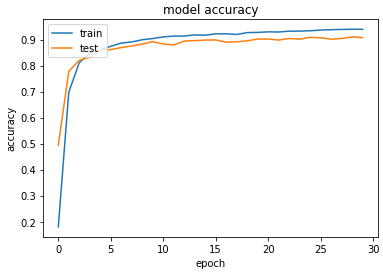
\includegraphics[width=\textwidth]{figures/Original/acc.png}
    \end{subfigure}
    \begin{subfigure}[b]{0.2\textwidth}
        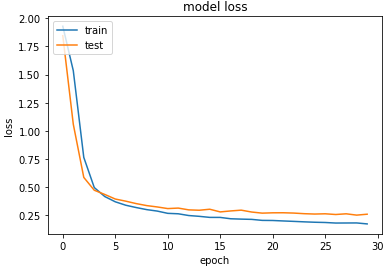
\includegraphics[width=\textwidth]{figures/Original/loss.png}
    \end{subfigure}
    
    \caption{\centering
    original models loss/accuracy in each epoch
    }
    \label{fig:original}
\end{figure}





\begin{figure}
    \centering
    \begin{subfigure}[b]{0.2\textwidth}
        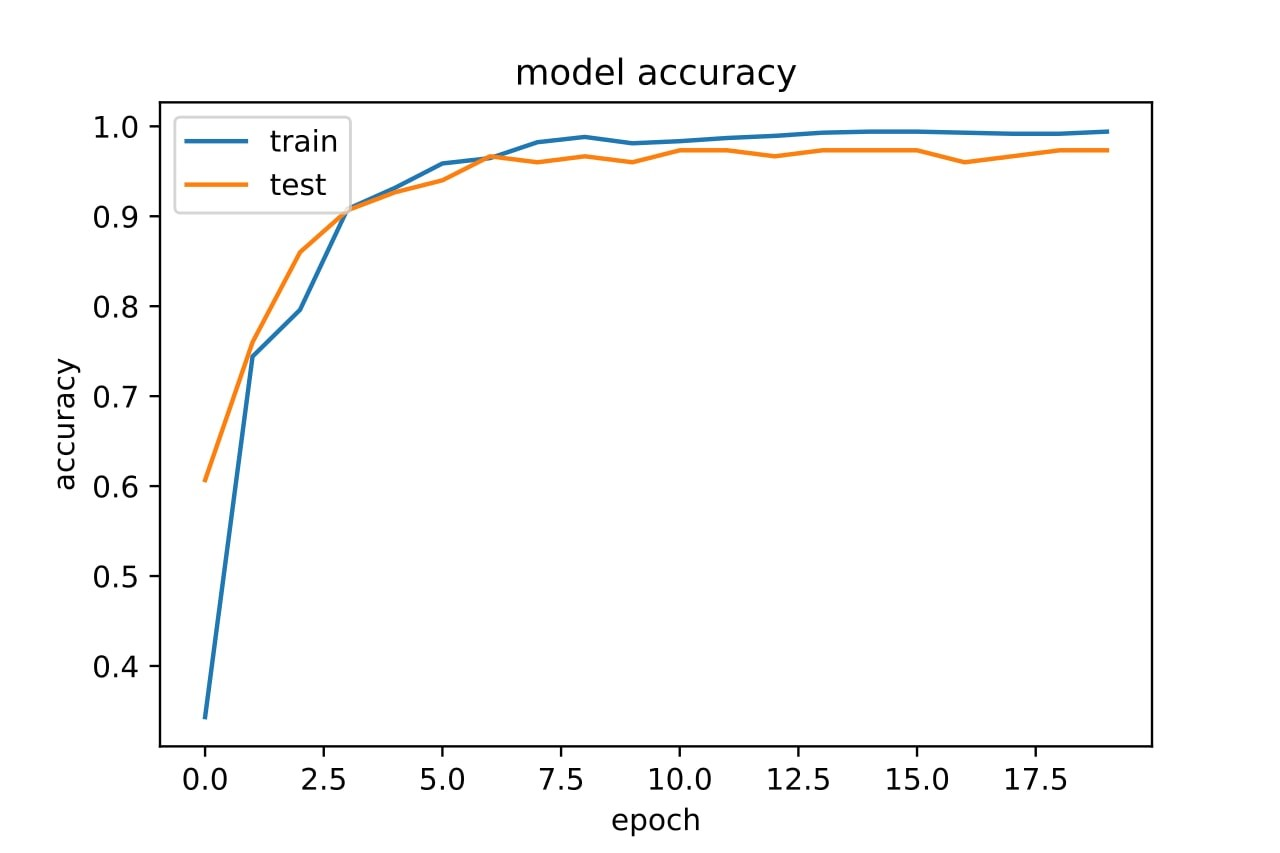
\includegraphics[width=\textwidth]{figures/Opt_RT/acc.jpg}
    \end{subfigure}
    \begin{subfigure}[b]{0.2\textwidth}
        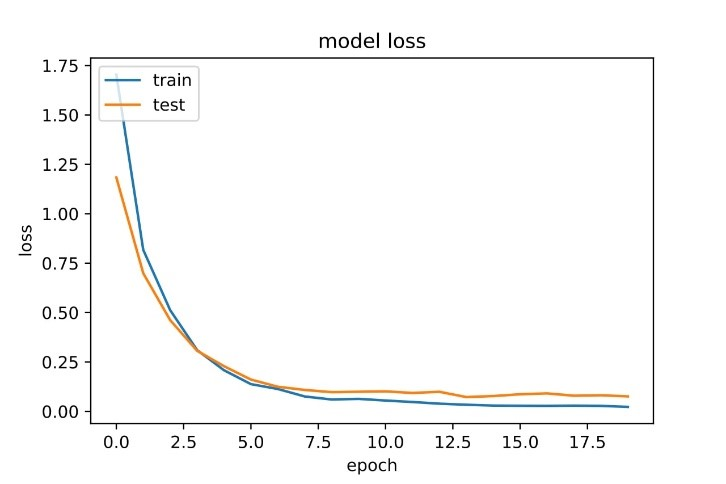
\includegraphics[width=\textwidth]{figures/Opt_RT/loss.jpg}
    \end{subfigure}
    
    \caption{\centering
    optimized models loss/accuracy in each epoch in real-time mode
    }
    \label{fig:org_rt}
\end{figure}








\begin{figure}
    \centering
    \begin{subfigure}[b]{0.2\textwidth}
        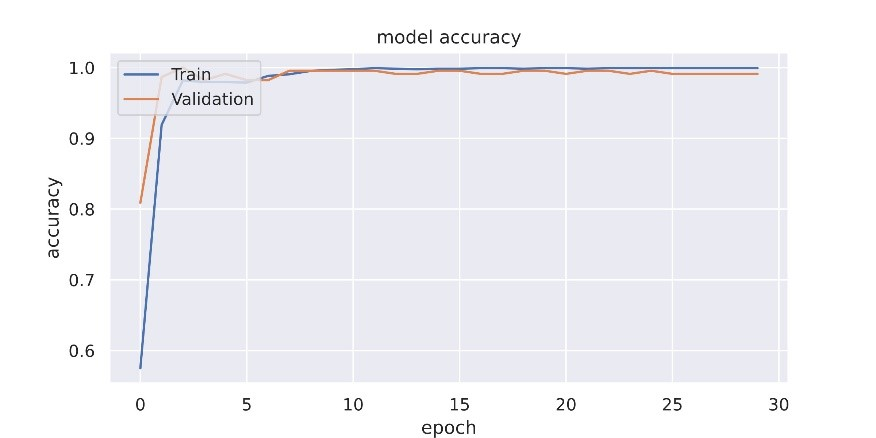
\includegraphics[width=\textwidth]{figures/Opt_OF/acc.jpg}
    \end{subfigure}
    \begin{subfigure}[b]{0.2\textwidth}
        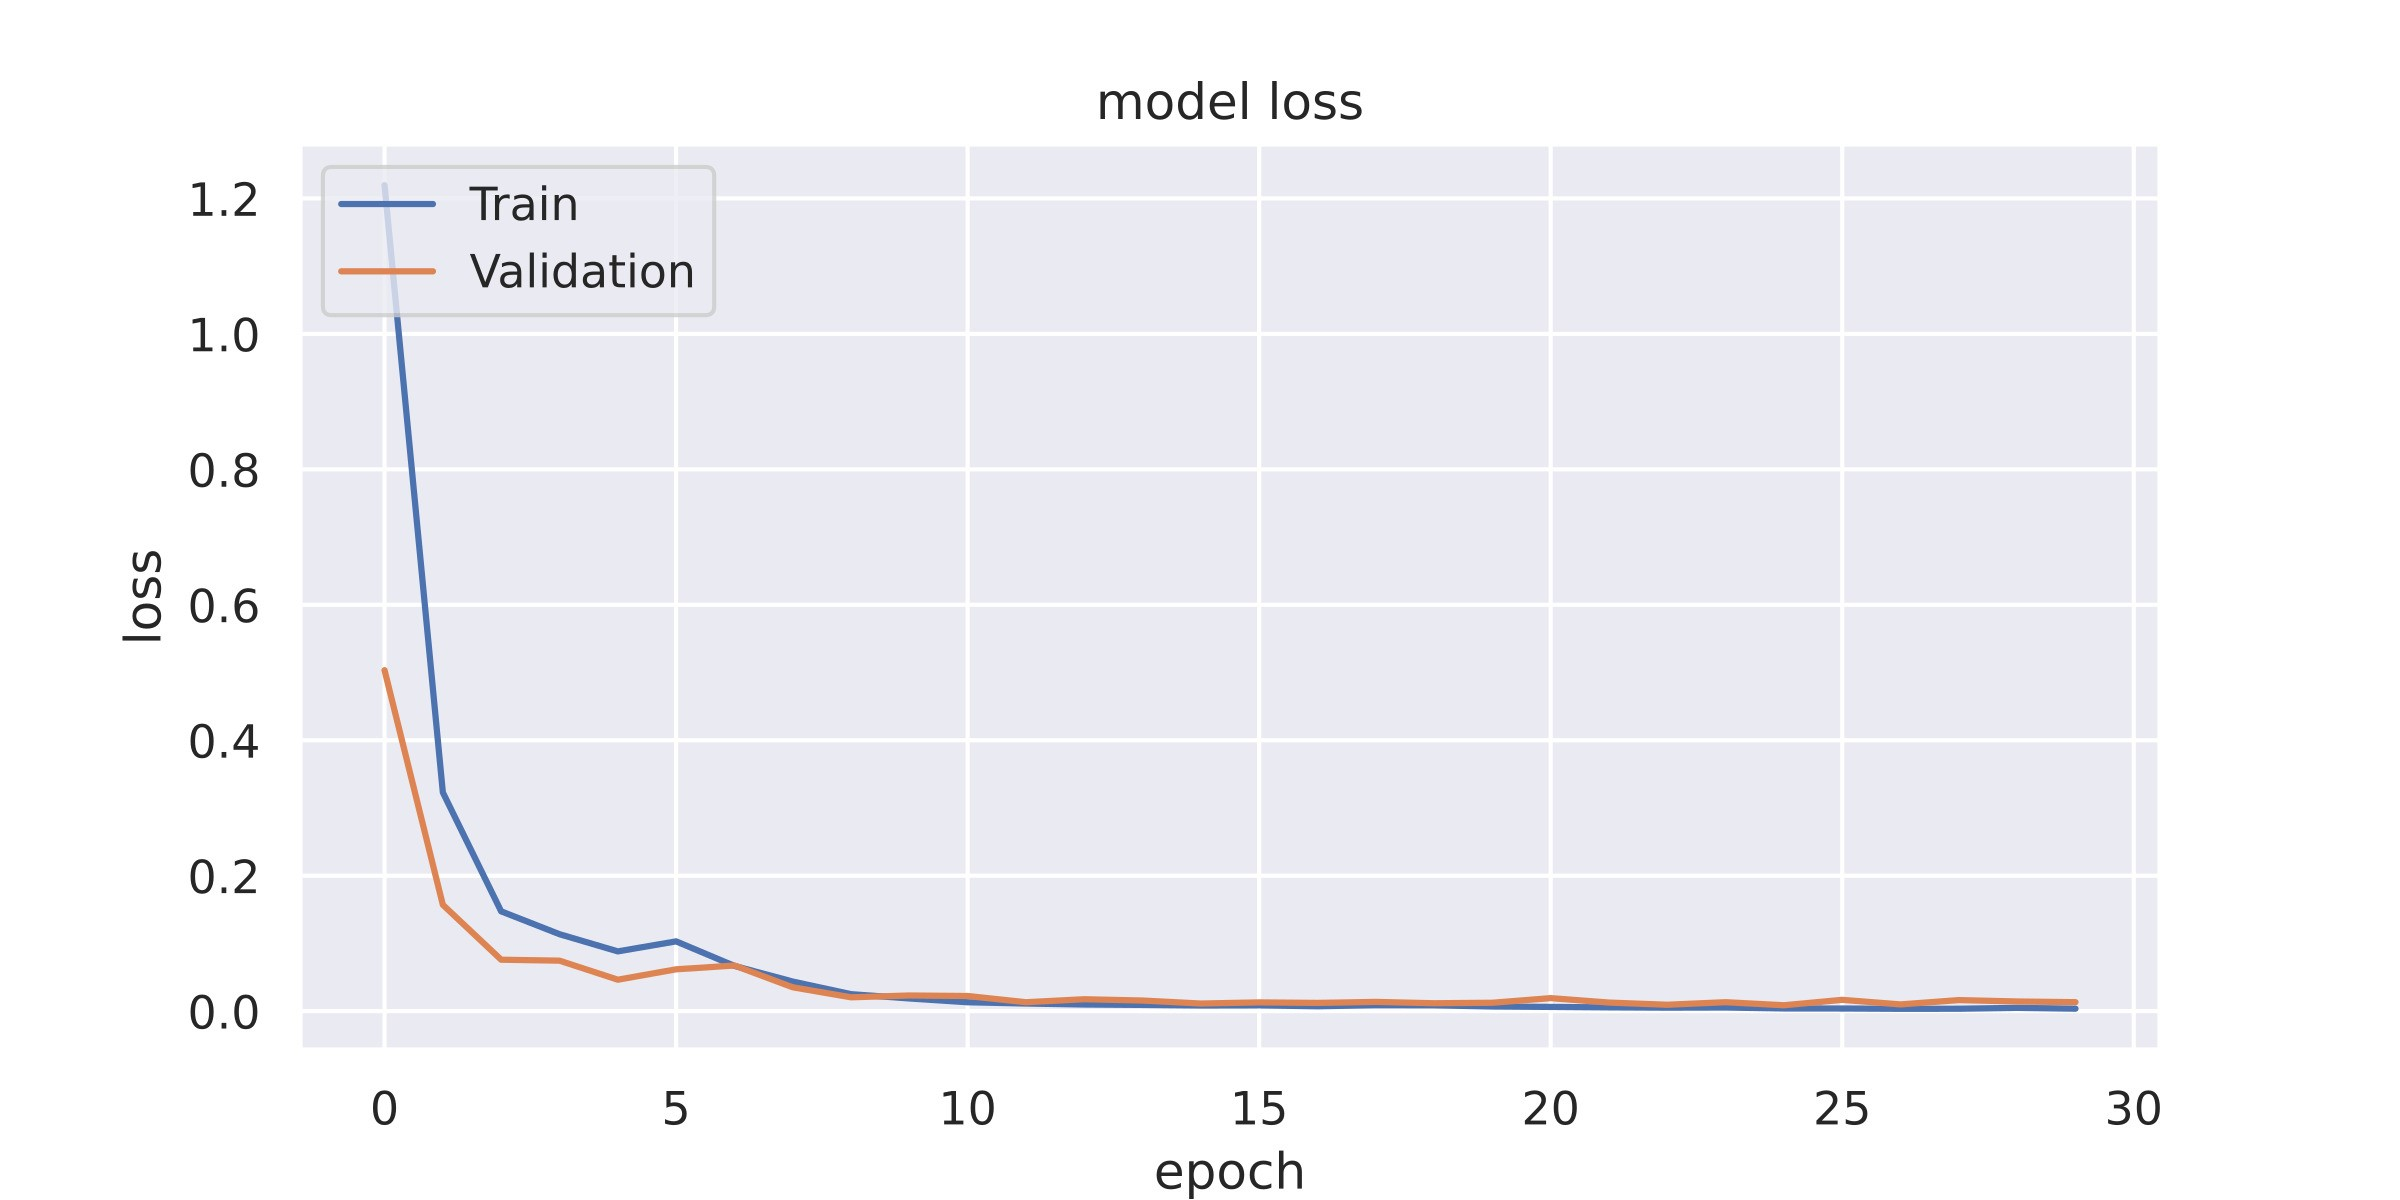
\includegraphics[width=\textwidth]{figures/Opt_OF/loss.jpg}
    \end{subfigure}
    
    \caption{\centering
    optimized models loss/accuracy  in each epoch in offline mode
    }
    \label{fig:org_of}
\end{figure}